\documentclass[presentation]{beamer}

\usepackage{tikz}
\usetikzlibrary{positioning,calc}
\usetikzlibrary{shapes.geometric}
\usetikzlibrary{backgrounds}% only to show the bounding box
\usetikzlibrary{shapes,arrows}
\usepackage{pgfplots}
\usepackage{pgfplotstable}
\usetikzlibrary{pgfplots.groupplots}
\pgfplotsset{compat=1.12}
\usepackage{appendixnumberbeamer}
\usepackage{amsmath}
\date{8th June 2016}
\usetheme{metropolis}

\pgfplotscreateplotcyclelist{decent cycle}{%
  {blue, mark=*, mark options={fill=blue},
    mark size=2pt},
  {cyan, mark=square*, mark options={fill=cyan},
    mark size=2pt},
  {magenta, mark=triangle*, mark options={fill=magenta},
    mark size=3pt},
  {blue, mark=*, mark options={fill=blue},
    mark size=2pt},
  {cyan, mark=square*, mark options={fill=cyan},
    mark size=2pt},
  {magenta, mark=triangle*, mark options={fill=magenta},
    mark size=3pt},
}

\pgfplotsset{
  decent/.style={
    cycle list name=decent cycle,
  }
}
\renewcommand{\vec}[1]{\ensuremath{\boldsymbol{#1}}}
\newcommand{\ddt}[1]{\frac{\partial #1}{\partial t}}
\newcommand{\zhat}{\hat{\vec{z}}}
\newcommand{\W}{\ensuremath{\mathbb{W}}}

\DeclareMathOperator{\grad}{grad}
\let\div\relax
\DeclareMathOperator{\div}{div}
\DeclareMathOperator{\curl}{curl}
\newcommand{\vsubset}[1]{\rotatebox[origin=c]{90}{\ensuremath{\subset}}}
\author{Lawrence Mitchell\inst{1}}
\institute{\inst{1}Departments of Computing and Mathematics, Imperial
  College London}

\graphicspath{{./\jobname.figures/}}

\newcommand{\arxivlink}[2]{%
  \href{http://www.arxiv.org/abs/#1}%
  {{\small\texttt{arXiv:\,#1\,[#2]}}}%
}
\usepackage[url=false,
            doi=true,
            isbn=false,
            style=authoryear,
            firstinits=true,
            uniquename=init,
            backend=biber]{biblatex}

\setbeamertemplate{bibliography item}{}
\renewcommand{\bibfont}{\footnotesize}
\addbibresource{references.bib}

\setlength{\bibitemsep}{1ex}

\renewbibmacro{in:}{}
\DeclareFieldFormat[article]{volume}{\textbf{#1}}
\DeclareFieldFormat{doi}{%
  doi\addcolon%
  {\scriptsize\ifhyperref{\href{http://dx.doi.org/#1}{\nolinkurl{#1}}}
    {\nolinkurl{#1}}}}
\AtEveryBibitem{%
\clearfield{pages}%
\clearfield{issue}%
\clearfield{number}%
}

\usepackage{minted}

\title{Firedrake: automating the finite element method by composing
  abstractions}

\begin{document}
\maketitle
\begin{frame}
  \frametitle{Firedrake team}
  David Ham, Mikl\'os Homolya, Fabio Luporini, Gheorghe-Teodor Bercea,
  Paul Kelly (Imperial College London)\\
  Andrew McRae (University of Bath)\\
  Florian Rathgeber (ECMWF).

  \url{www.firedrakeproject.org}\\
  \url{github.com/firedrakeproject/firedrake}
\end{frame}

\begin{frame}
  \frametitle{Automated finite elements?}
  How do we develop models?

  \begin{itemize}
  \item Choose equations
  \item Pick method/discretisation
  \item Decide on implementation language, target architecture?
  \item Write code to implement method
  \end{itemize}
\end{frame}

\begin{frame}
  \frametitle{Traditional implementation}

Numerics intertwined with implementation

Difficult to programmatically apply optimisations

Mathematical structure often lost
\end{frame}

\begin{frame}
  \frametitle{Generative programming}
  Capture appropriate abstraction.

  Synthesise low-level code with special-purpose compilers
\end{frame}

\begin{frame}
  \frametitle{An example}
  
  \begin{block}{The Monge-Amp\`ere equation}
    \begin{align*}
      \sigma &= D^2 u,\\
      \det(I + \sigma) &= f.
    \end{align*}
    Weak formulation, find $(u, \sigma) \in V \times \Sigma$ s.t.
    \begin{align*}
   \int_\Omega \tau:(\sigma + D^2u)\,\text{d}x
   - \int_{\partial\Omega} \tau_{12}n_2u_x + \tau_{21}n_1u_y\,\text{d}s
     =0, \quad \forall \tau \in \Sigma\\
   \int_\Omega v\det(I + \sigma)\,\text{d}x = \int_\Omega
   fv\,\text{d}x \quad \forall v \in V.
    \end{align*}
  \end{block}
\end{frame}
\begin{frame}[fragile]
  \frametitle{Implementation}
\begin{minted}[fontsize=\tiny]{python}
from firedrake import *
mesh = UnitSquareMesh(100, 100, quadrilateral=True)
V = FunctionSpace(mesh, "CG", 2)
Sigma = TensorFunctionSpace(mesh, "CG", 2)
W = V*Sigma
f = Function(V)
v, tau = TestFunctions(W)
w = Function(W)
u, sigma = split(w)
n = FacetNormal(mesh)
I = Identity(mesh.geometric_dimension())

F = (inner(sigma, tau)*dx - (det(I + sigma) - f)*v*dx +
     inner(div(tau), grad(u))*dx -
     (tau[0, 1]*n[1]*u.dx(0) + tau[1, 0]*n[0]*u.dx(1))*ds)

solve(F == 0, w, ...)
\end{minted}
\end{frame}

\begin{frame}[standout]
  Say \emph{what}, not \emph{how}.
\end{frame}
\begin{frame}
  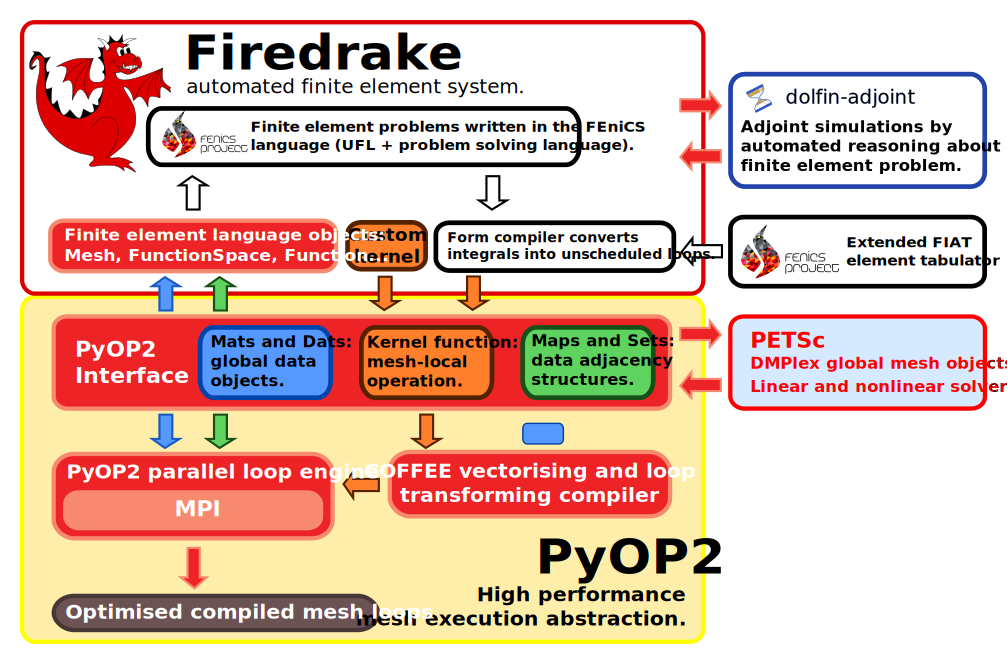
\includegraphics[width=\textwidth]{firedrake-stack}
\end{frame}

\begin{frame}
  \frametitle{Form compilation}
  No single optimal scheduling of loop nests that occur in finite
  element integration.  Depends on degree, form complexity, basis
  function structure.

  \cite{Luporini:2016} \arxivlink{1604.05872}{cs.MS}
\end{frame}

\begin{frame}
  \frametitle{Mesh iteration}
  Mesh-based solvers execute \emph{local} operation over mesh
  gathering data with some \emph{stencil}.

  PyOP2 captures these iterations and manages the execution.

  Most naive implementation just does ``the iteration you would have
  written''.

  But, we can do more.  In particular, unstructured mesh loop-tiling.
\end{frame}

\begin{frame}
  \frametitle{Solvers}
  
\end{frame}
\appendix
\begin{frame}
  \frametitle{References}
  \printbibliography[heading=none]
\end{frame}
\end{document}
